\section{Description of MAC model}


A MAC network is an end-to-end differentiable architecture primed to perform an explicit multi-step reasoning process, by stringing together p recurrent MAC cells, each responsible for performing one reasoning step. Given a knowledge base K (for VQA, an image) and a task description q (for VQA, a question), the model infers a decomposition into a series of p reasoning operations that interact with the knowledge base, iteratively aggregating and manipulating information to perform the task at hand. It consists of three components: (1) an input unit, (2) the core recurrent network, composed out of p MAC cells, and (3) an output unit, all described below.

\begin{figure}[htbp]
	\centering
	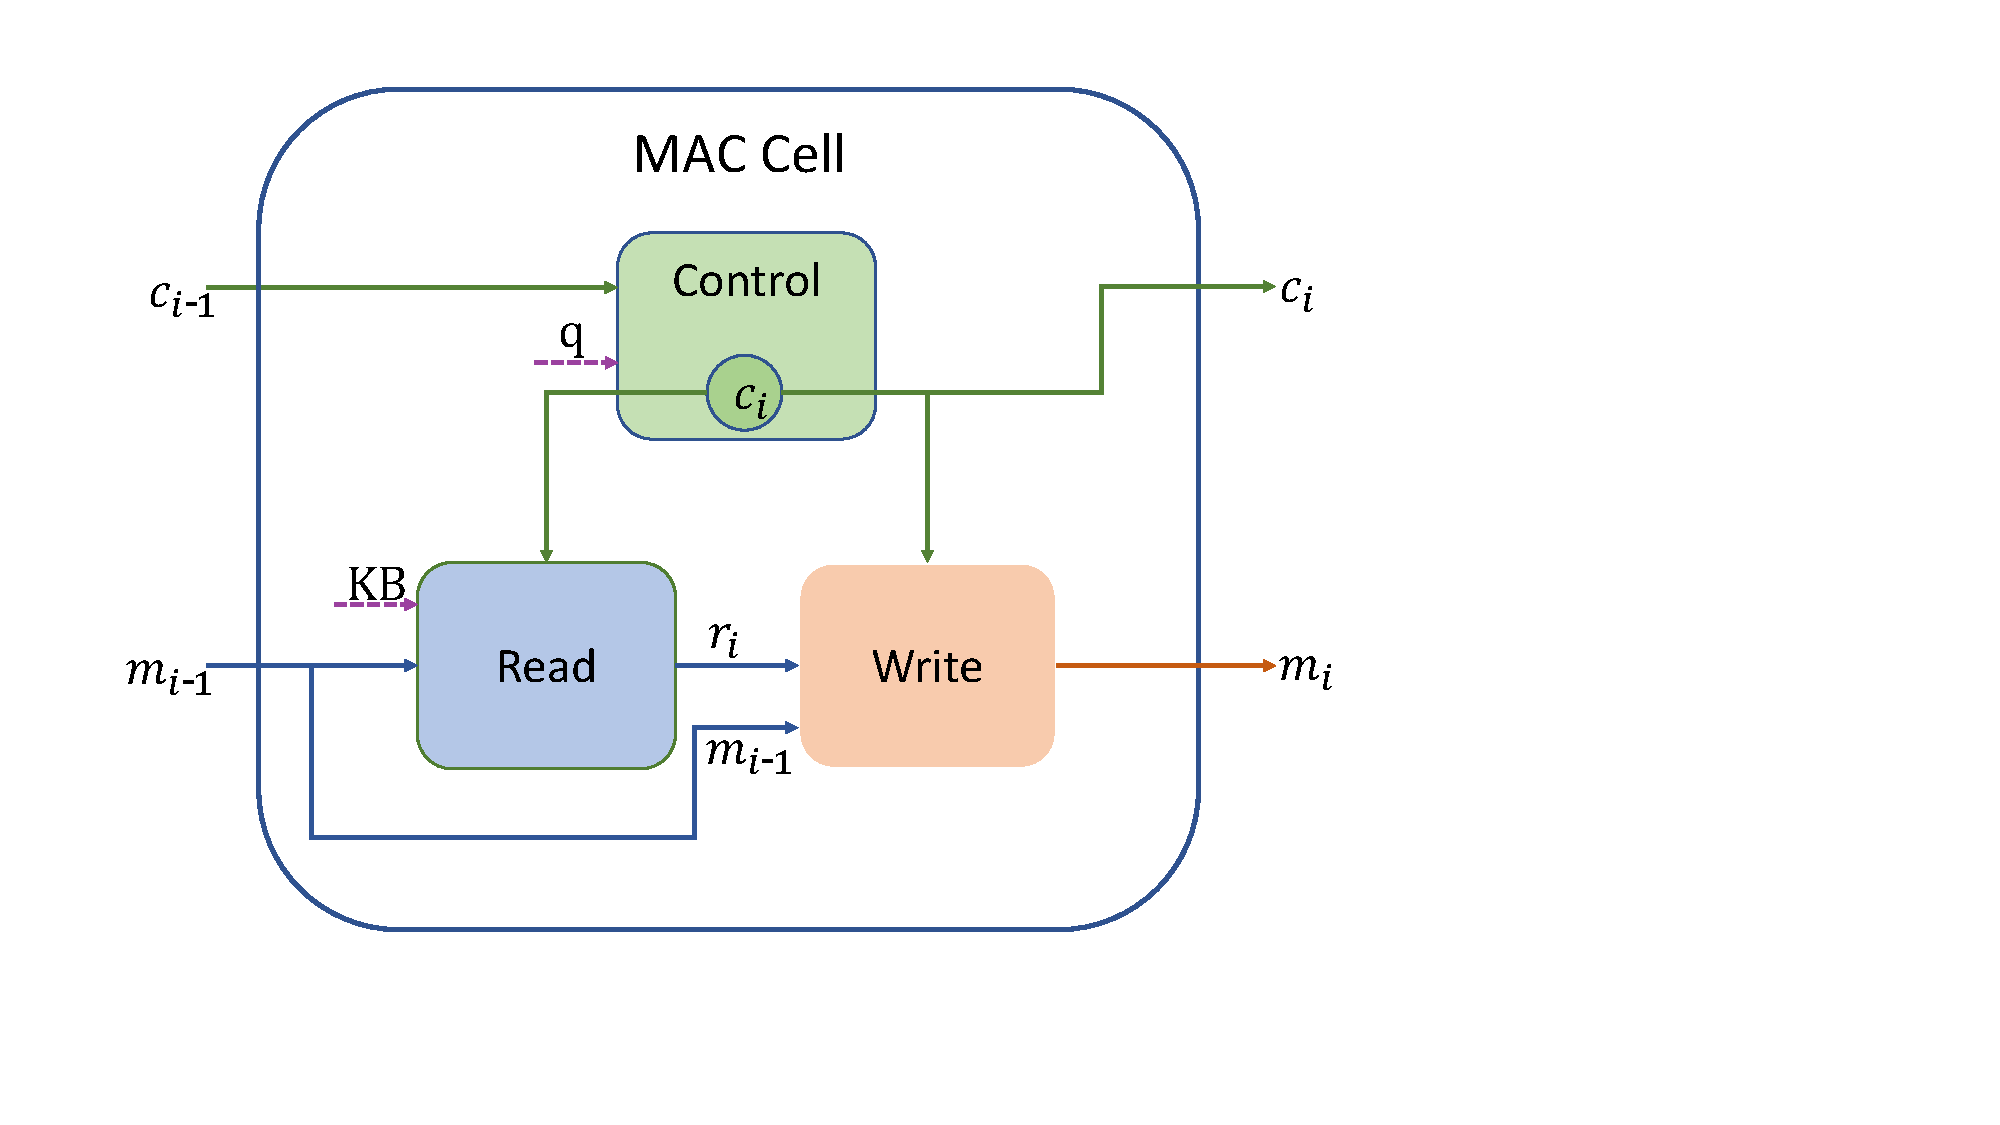
\includegraphics[width=0.7\textwidth]{img/mac_cell.pdf}
	\caption{The Mac Cell. The MAC recurrent cell consists of a control unit, read unit, and write unit, that operate over dual control and memory hidden states. The control unit successively attends to different parts of the task description (question), updating the control state to represent at each timestep the reasoning operation the cell intends to perform. The read unit extracts information out of a knowledge base (here, image), guided by the control state. The write unit integrates the retrieved information into the memory state, yielding the new intermediate result that follows from applying the current reasoning operation.}
	\label{fig:core_concepts}
\end{figure}

